\section{Search for Same Sign Top Quark Pair Production}
\label{sec:samesign}

This analysis is based on the approved same-sign dilepton search documented in AN 2010/247 v6 \cite{ssnote1}
and corresponds to an integrated luminosity of 35 pb$^{-1}$.
In that analysis we searched for events with two isolated same sign leptons, two or more jets, and MET ($\met$).
This final state is exactly the final state that one would expect from top-top production with 
both top quarks decaying as $t\rightarrow Wb$, $W\rightarrow \ell \nu$.

\subsection{Event Selection}

In AN 2010/247 we presented event yields and background expectations for several event selections.  
One of those event selections is very similar to that of the $t\bar{t}$ (opposite sign) dilepton 
cross-section analysis \cite{topxsection}, 
and thus it is the appropriate selection for a top-top pair search.  
Briefly, this selection consists of

\begin{itemize}
	\item Two same sign leptons of $p_T>20$ GeV, $|\eta|<2.4$
	\item Two jets of $p_T>30$ GeV, $|\eta|<2.4$
	\item $\met >20$ GeV ($e\mu$) or $\met>30$ GeV ($ee$ or $\mu\mu$)
\end{itemize}

\noindent More details are found in Reference~\cite{ssnote1}.

\subsection{Event Yields and Background}
\label{sec:ssyields}

The results of the search in this kinematical region are 
summarized in Table 6 of AN 2010/247 v6 \cite{ssnote1}, 
which is reproduced below as Table \ref{tab:ssyields}.

The data-driven background prediction is based on a combination 
of estimating ``fake leptons''~\cite{fakenote} (FakeRate) 
and electrons reconstructed with the wrong sign~\cite{ssnote1} (Charge FlipRate). 
The probability for muons to be reconstructed with the wrong sign 
in the relevant momentum range is negligible.


%%% Commented out DLE
%This section summarizes the results of the search for same sign $tt$
%pair production in the di-lepton channel. We use two data-driven methods 
%to estimate background characterized by the presence of two isolated high $P_T$ same 
%sign leptons, $\met$, and significant hadronic activity. For the purpose of this note we 
%restrict ourselves to the $ee$, $e\mu$, and $\mu\mu$ final states, {\em i.e.}, we do not 
%consider $\tau$'s, except in the case that the $\tau$ decays leptonically. 
%%%
%As we will show in Section~\ref{sec:ssyields}, for this modified baseline selection is similar to
%the published opposite sign di-lepton pair production cross section paper~\cite{topxsection}, where the main 
%background is from SM \ttbar decays. The data-driven background prediction is based on a combination 
%of estimating ``fake leptons''~\cite{fakenote} (FakeRate) and electrons reconstructed with the 
%wrong sign~\cite{ssnote1} (Charge FlipRate). The probability for muons to be reconstructed with 
%the wrong sign at the relevant momenta is negligible.

%after applying the event selections
%described in Section~\ref{sec:eventselection} to the datasets described in Section~\ref{sec:datasamples} 
%are detailed below. The final event yields also include the systematic uncertanities of
%the method used.

\vspace{6 mm}
\begin{table}[htb]
\begin{center}
\begin{tabular}{|c|c|c|c|c|}
\hline
Sample & $e^{\pm}e^{\pm}$    & $\mu^{\pm}\mu^{\pm}$ & $e^{\pm}\mu^{\pm}$      & total \\ \hline
% all the MCs
\hline
DY  & 0.00000 $\pm$ 0.00000 & 0.00000 $\pm$ 0.00000 & 0.00000 $\pm$ 0.00000 & 0.00000 $\pm$ 0.00000 \\ 
t$\overline{t}$  & 0.03700 $\pm$ 0.01170 & 0.04440 $\pm$ 0.01282 & 0.09250 $\pm$ 0.01850 & 0.17391 $\pm$ 0.02537 \\ 
wjets  & 0.10860 $\pm$ 0.10860 & 0.00000 $\pm$ 0.10860 & 0.00000 $\pm$ 0.10860 & 0.10860 $\pm$ 0.18810 \\ 
tw  & 0.00079 $\pm$ 0.00079 & 0.00079 $\pm$ 0.00079 & 0.00475 $\pm$ 0.00194 & 0.00634 $\pm$ 0.00224 \\ 
single top t-ch.  & 0.00138 $\pm$ 0.00138 & 0.00000 $\pm$ 0.00138 & 0.00276 $\pm$ 0.00195 & 0.00415 $\pm$ 0.00276 \\ 
single top s-ch.  & 0.00000 $\pm$ 0.00012 & 0.00035 $\pm$ 0.00020 & 0.00023 $\pm$ 0.00016 & 0.00058 $\pm$ 0.00028\\ 
ww  & 0.00000 $\pm$ 0.01219 & 0.00000 $\pm$ 0.01219 & 0.01219 $\pm$ 0.01219 & 0.01219 $\pm$ 0.0211 \\ 
wz  & 0.01109 $\pm$ 0.00784 & 0.01109 $\pm$ 0.00784 & 0.07207 $\pm$ 0.01999 & 0.09425 $\pm$ 0.02286 \\ 
zz  & 0.00000 $\pm$ 0.00178 & 0.00178 $\pm$ 0.00178 & 0.00535 $\pm$ 0.00309 & 0.00713 $\pm$ 0.00356 \\ 
\hline
Total MC  & 0.15886 $\pm$ 0.10952 & 0.05841 $\pm$ 0.01515 & 0.18986 $\pm$ 0.03012 & 0.40713 $\pm$ 0.11459 \\
\hline\hline
data  (35 pb$^{-1}$)     & 0  &  0  & 2  & 2      \\ \hline
fake rate prediction & & & & \\ \hline
single fake   & 0.47105 $\pm$ 0.33308 & 0.12058 $\pm$ 0.12058 & 1.05798 $\pm$ 0.48320 & 1.64961 $\pm$ 0.59914 (8 evts) \\
double fake   & 0.00000 $\pm$ 0.24180 & 0.00000 $\pm$ 0.02086 & 0.00000 $\pm$ 0.07102 & 0.00000 $\pm$ 0.25288 (0 evts) \\
fake prediction & 0.47105 $\pm$ 0.41159 & 0.12058 $\pm$ 0.12237 & 1.05798 $\pm$ 0.48839 & 1.64961 $\pm$ 0.65032 \\
\hline
flip rate prediction & $0.06\pm 0.01$ & 0 & $0.02\pm 0.003$ & $0.08\pm 0.01$ \\ \hline\hline
total data driven prediction & $0.54\pm 0.48$ & $0.13\pm 0.14$ & $1.07\pm 0.72$ & $1.74\pm 1.05$ \\ \hline
total MC driven prediction & $0.01\pm 0.01$ & $0.01\pm 0.01$ & $0.08\pm 0.04$ & $0.10\pm 0.05$ \\\hline\hline
total bkg prediction & $0.55\pm 0.48$ & $0.14\pm 0.14$ & $1.15\pm 0.7$ & $1.8\pm 1.1$ \\\hline
\end{tabular}
\caption{\protect Data and Monte Carlo yields for the same sign di-leptons with $P_T >20$\ GeV
from Reference~\cite{ssnote1}.  Note that this Table inludes $\ell^+\ell^+$ as well
as $\ell^-\ell^-$; Both signal events are $e^+\mu^+$.
Uncertainties in the lower three rows also include the systematic 
uncertanities on the method used.\label{tab:ssyields} }
\end{center}
\end{table}

The event yields have the following characteristics:

\begin{itemize}
\item We do not consider rare processes such as $qqW^\pm W^\pm, WWW, t\bar{t}W$, double parton $W^\pm W^\pm$, which are 
negligibly small~\cite{ssnote1}.
% \item We found small contributions (0.01 events) from conversion of prompt photons in $W/Z\gamma$ using MC and are
% not considered in order to avoid double counting in the single fake contributions.
\item The diboson backgrounds $WW, WZ, ZZ$ are taken from the MC as an additional background estimate. This contribution
is tabulated as the total MC driven predicition.
\item The prediction from fake rates includes the systematic error of 50\%. 
\item The flip rate prediction also includes an additional systematic error of 50\% based on statistics of the same
sign events observed in the control region~\cite{ssnote1}.
\item The systematic errors are added when propagating the fake/flip rates into total data-driven predictions.
\item All MC driven predictions also assume a flat 50\% systematic error.
\end{itemize}

The dominant SM contribution is from \ttbar decays. The total estimated background 
is obtained after the application of Fake and Charge Flip rates 
to the dilepton dataset\cite{ssnote1}. 
The data yield is in good agreement with the background prediction. 
% from both MC as 
% well as the data driven predictions. 

We take the results of Table \ref{tab:ssyields} with one important modification: 
since we are interested in $tt$ production and not $\bar{t}\bar{t}$ production,
we only consider $\ell^{+}\ell^{+}$ events.  
Thus the background estimates in Table \ref{tab:ssyields} have to be divided by two.
Strictly speaking the W$+$jets background, which according to MC is about 25\%
of the total, is not completely charge symmetric.  
This background is calculated in a data-driven 
way using the fake rate method.  We have repeated the fake rate calculation
of Table~\ref{tab:ssyields} for positive leptons only; the result is 
0.67 $\pm$ 0.34 (stat.) $\pm$ 0.28 (sys.) events, which is consistent with being one half of the estimate for both
positive and negative leptons of Table~\ref{tab:ssyields}  (1.65 events divided
by 2 = 0.8).

Both observed events in Table \ref{tab:ssyields} have positive leptons.  
Then, the bottom line yield and background prediction is: 
two events observed and $0.9 \pm 0.6$ expected background, 
which corresponds to one half the background of Table \ref{tab:sm_preditcion}.
Thus, we see no statistically significant evidence for $pp \to tt$.


% One of the key components of same-sign top pair search is the fact that the final state includes  
% includes mainly one type of sign. 
% For example, in the t-channel exchange: $ uu \rightarrow tt \rightarrow l^+ l^+ \mu \nu b b$ only positively charged leptons are involved. 
% The quark quark, $\bar{u}\bar{u}$ scattering is highly suppressed due to the parton luminosities, thus we do not expect any significant contribution 
% from negatively charged leptons. 
% Given that the data driven methods are robust against any given choice of lepton charge~\cite{fakenote1}, we use half of the total background prediction for this search.


% The results is summarized in Table~\ref{tab:sm_preditcion}.

\begin{table}[hbt]
\begin{center}
\begin{tabular}{|l|c|}\hline
Same sign dileptons & Event yield \\ \hline
Total Observed & 2 \\
Total Predicted & 0.9 $\pm$ 0.55 \\
\hline
\end{tabular}
\caption{ Observed and predicted number of events passing the event selection in 35 pb$^{-1}$ of integrated luminosity. 
The uncertainty also includes systematic errors.\label{tab:sm_preditcion}}
\end{center}
\end{table}

%The ``anatomy'' of the 2 observed event is discussed in the appendix.
% Although the observed events have two positively charged 
% di-leptons, we do not consider this a significant deviation from the prediction.

\subsection{Systematic Uncertainties on the Acceptance}
\label{sec:sssystematics}

The methods used to determine the systematic uncertainties are discussed in Reference~\cite{ssnote1}.
For lepton selections, we take the result from ~\cite{ssnote1}.
We have recalculated the systematic uncertainties due to ISR/FSR, PDFs, and jet energy scale
appropriate to the $pp \to tt$ process.  The results are 
summarized 
in Table \ref{tab:systSumm}.

\begin{table}[h]
\begin{center}
\begin{tabular}{lcccc}\hline
Source 					& $ee$		& $\mu\mu$		& $e\mu$			& all \\ \hline
Lepton selection			& 11.8\%		& 10.6\%		& 10.8\%			& 10.7\% \\
Energy scale				& 8\%		& 8\%		& 8\%			& 8\% \\
ISR/FSR and PDF				& 3\%		& 3\%		& 3\%			& 3\% 	\\
Total without luminosity		& 14.6\%		& 13.6\%		& 13.8	& 13.7\%	\\ \hline
Integrated luminosity			& 4\%		& 4\%		& 4\%			& 4\%	\\ \hline
Total & 15\% & 14\% & 14\%  & 14\% \\
%%% Total & 13.6\% & 12.4\% & 12.5\%  & 12.5\% \\
\hline
\end{tabular}
\caption{\small\label{tab:systSumm}Summary of systematic uncertainties on the signal selection and
expectation. Reported values are fractional, relative to the total cross section.}
\end{center}
\end{table}

\section{Results}
\label{sec:ssresults}

In absence of any significant deviation from the predicted background we set 95\% CL. on the number of observed events. 
Two statistical methods have been used for the upper limit. 
Both methods assume the uncertainties on signal and background are un-correlated and use a log-normal distribution for error pdfs. 

The first method used to compute the upper limit is based on Bayesian statistics~\cite{bayesian}.
A posterior probability $p(r)$ is used as a function of the signal strength $r = \sigma/\sigma_{SM}$ 
assuming a uniform prior for $r$ integrating the nuisance parameters associated to the uncertainties.
The upper limit at 95\% confidence level is then determined by integrating $p(r)$ to determine $r'$, 
which satisfies $\int_{r'}^{\inf} p(r) dr = 0.05$.

We use the hybrid frequentist-bayesian $CLs$ approach~\cite{CLS} as the second method. 
Although the two statistical approaches are not equivalent, in this case we get similar results. 

\begin{itemize}
\item Upper limit at 95\% CL. with 14\% signal systematic error using Bayesian approach = 5.7  
\item Upper limit at 95\% CL. with 14\% signal systematic error using $CLs$ = 5.6  
\end{itemize}

We use 5.7 events as the upper limit for the rest of this document. 
This corresponds to a 95\% CL. upper limit on the effective cross section for new processes, 
including the effects of experimental acceptance and efficiency, of 0.3 pb for the same sign di-lepton channel.

Fig.~\ref{fig:sstopexclusion} shows the exclusion region at 95\% CL. as a function of $Z'$ mass and the right-handed coupling, $f_R$. 
LO signal cross sections are used for this study. 
The limit on t-channel exchange diagrams $tt$ covers a significant region as a function of the $Z'$ mass.
In most cases it does not favor large values of the coupling $f_R$. 
As expected, when using 35 pb$^{-1}$ of integrated luminosity the limit on $ttj$ production is weak and 
only excludes up to $m_Z' \sim 500$ GeV for higher values of $f_R$. 

Fig.~\ref{fig:sstopcombexclusion} shows the combined exclusion region ($tt$ and $ttj$) at 
95\% CL. as a function of $Z'$ mass.  The combined exclusion is dominated by $tt$.
% The region excludes a large range of the $Z'$ mass for various 
% choices of the coupling for same sign top 
% production at the LHC

\begin{figure}[htb]
\begin{center}
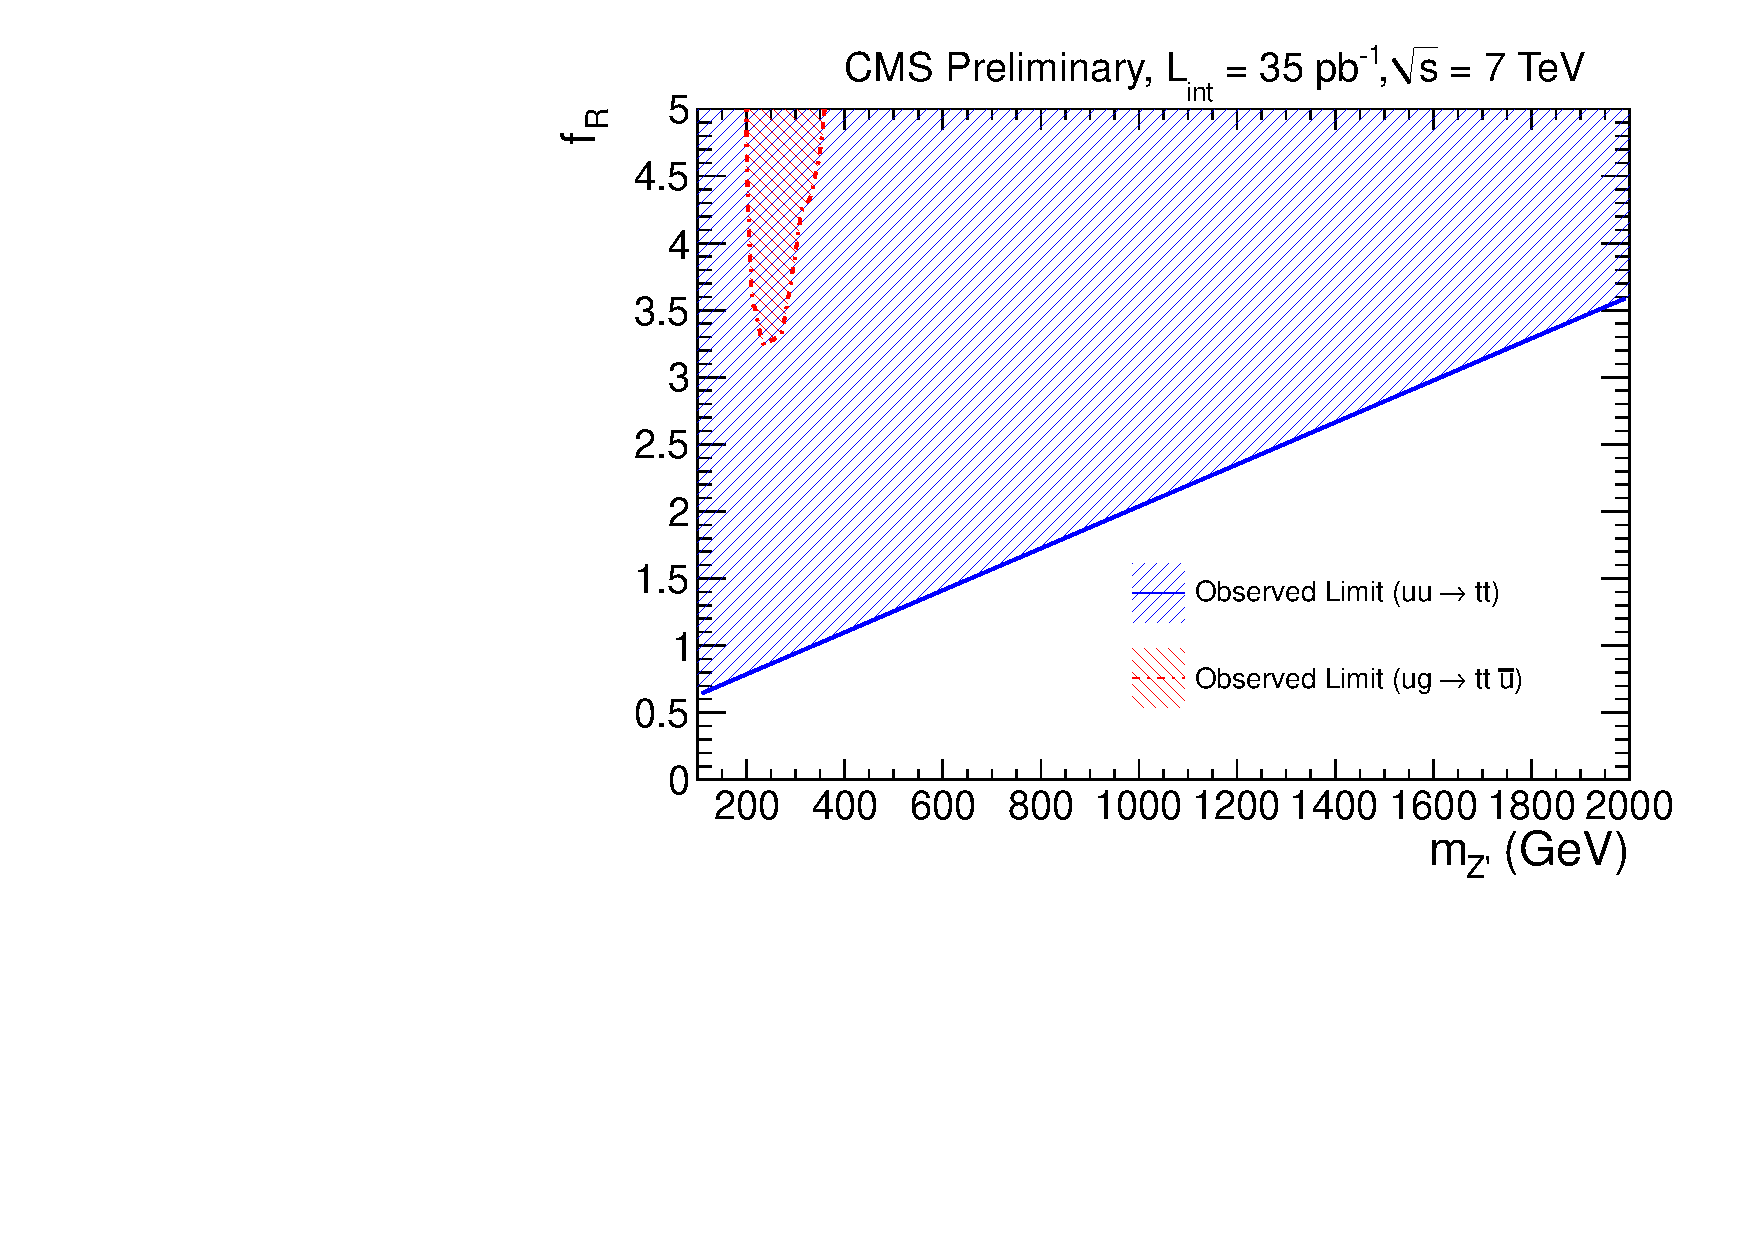
\includegraphics[width=0.7\linewidth]{figs/sstop_result.pdf}
\caption{ The exclusion region at 95\% CL. as a function of $Z'$ mass for various choices of the 
right-handed coupling, $f_R$. The solid lines represents regions due to t-channel exchange, where
as the dotted line excludes the assumptions on $ttj$ pair production. For the renormalization and factorization 
scales, $\mu$ is set to the top mass. \label{fig:sstopexclusion}}
\end{center}
\end{figure}

\begin{figure}[htb]
\begin{center}
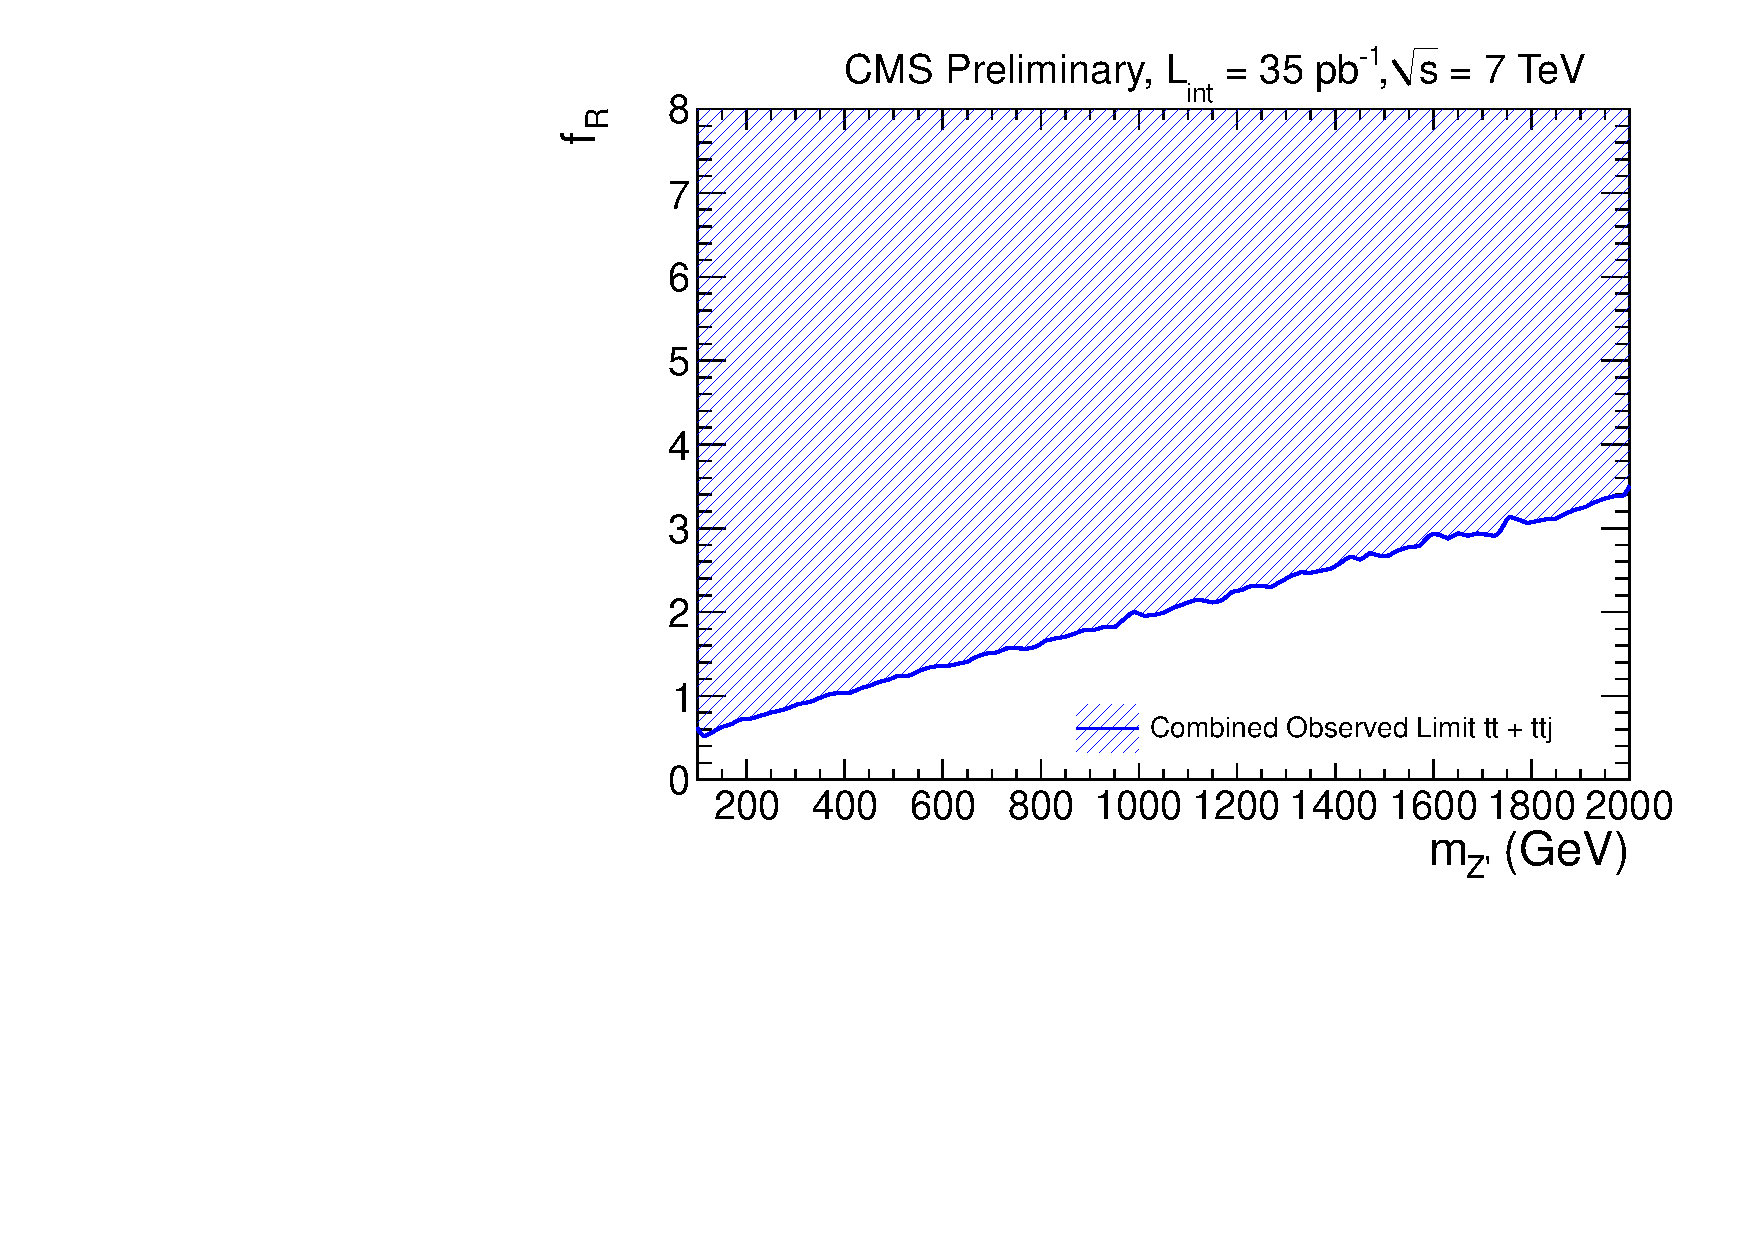
\includegraphics[width=0.7\linewidth]{figs/sscomb.pdf}
\caption{ The combined exclusion region at 95\% CL. as a function of $Z'$ mass for various choices of the 
right-handed coupling, $f_R$. Both t- and s-channel diagrams are added to get the combined exclusion limit
on same sign top production at the LHC. For the renormalization and factorization 
scales, $\mu$ is set to the top mass. \label{fig:sstopcombexclusion}}
\end{center}
\end{figure}
